\section{Espectro de radiofrecuencias}
De la página del Ente Nacional de Comunicaciones (ENACOM): "El Espectro Radioeléctrico es el conjunto de frecuencias que, conforme a la tecnología disponible, pueden ser empleadas para emitir ondas que permitan transportar información. La manera en cómo está atribuido el Espectro Radioeléctrico en nuestro país se puede consultar en el "Cuadro de Atribución de Bandas de Frecuencias de la República Argentina", al que abreviadamente se lo conoce como CABFRA."

El espectro es considerado un recurso natural, de carácter limitado,  sobre el cual el estado tiene soberanía. Por lo tanto, se lo divide en bandas atribuidas a distintos servicios y sistemas de comunicaciones. A continuación se presenta una figura con las atribuciones según el CABFRA. 

\begin{table}[H]
\begin{tabular}{|l|L{6cm}|L{6cm}|}
\hline
SERVICIO            & FRECUENCIAS DE OPERACIÓN                                                                                                                                                           & POTENCIA IRRADIADA                                                                                                                                 \\
\hline
Radiodifusión de AM & 535 - 1705 kHz                                                                                                                                                                     & Mín 100 W Máx 100 kW                                                                                                                               
\\
\hline
Radiodifusión de FM & 88 - 108 MHz                                                                                                                                                                       & Mín 30 W Max 100 kW                                                                                                                                \\
\hline
Radiodifusión de TV & TV abierta \textbf{VHF bajo:} 54 - 72 MHz (canales 2-4) 76 - 88 MHz (c. 5-6) \textbf{VHF alto:} 174 - 216 MHz (c. 7-13) \textbf{UHF} (en gral. TV codificada, o sea no abierta)512 - 806 MHz (21-69) & \textbf{VHF:} Mín 5 kw en estación autónoma, 50 W en repetidora. Máx 30 kW en transmisor irradiado hasta 150 kW \textbf{UHF} (codificado, área reducida):aprox. 25 W \\
\hline
Telefonía celular   & \textbf{SRMC/STM:} 869 - 894 MHz (base) 824 - 849 MHz (móvil) \textbf{PCS:} 1850 - 1910 MHz (móvil)1930 - 1990 MHz (base)                                                                            & Celdas en zona muy urbanizada: Aprox. 20 WZona rural: máx. 100 W                                                                                   \\
\hline
HF                  & Servicio fijo y móvil (en gral uso comercial): 2 - 30 MHzRadioaficionados:bandas en los rangos de 1,8 - 3,6 - 3,8 - 7 -10 - 14 - 18 - 21 - 25 y 29 MHz                             & Se especifica potencia pico de envolvente (la potencia media está unos 10 dB por debajo) Uso comercial: máx 160 WRadioafición: máximo 1,5 kW       \\
\hline
VHF y UHF           & \textbf{{[}MHz{]}}30 - 50138 - 174242 - 280340 - 399421 - 426443 - 490                                                                                                                      & Handies 6 W Móvil 40 WBase 60 WEstos son valores típicos                                                                                           \\
\hline
Móvil Marítimo      & \textbf{Rangos HF:} 4, 6, 8, 12, 16, 18, 22, 25 MHz \textbf{Rangos VHF}: 156, 0 - 157,5 /160,5 - 162 MHz                                                                                             & \textbf{HF}: aprox. 150 W pico de envolvente \textbf{VHF}: 25 W                                                                                                      \\
\hline
Móvil Aeronáutico   & \textbf{HF (AM)}: entre 2 y 30 MHz \textbf{VHF:} 108 - 118 MHz radionavegación (ILS, VOR)118 - 136 MHz comunicaciones móvil - tierra                                                                 & \textbf{HF}: hasta 400 W PEP (media 100 W) \textbf{VHF}: 20 W\\
\hline
 
\end{tabular}

\caption{Cuadro de Atribuci\'on de Bandas de Frecuencias de la Rep\'ublica Argentina (CABFRA)}
\label{tab:freq}
\end{table}

Considerando esta table, se buscó sintonizar una frecuencia que no perteneciera a una emisora de radio o TV.

\section{Banda FM}

El espectro FM está dividido en siete categorías (de la A a la G) según el radio de servicio. A continuación se presenta una tabla tomada de la página web oficial del ENACOM en la que se muestra la división de bandas por categorías.

\begin{table}[H]
\centering
\begin{tabular}{|c|c|}
\hline
CATEGORÍA & \begin{tabular}[c]{@{}l@{}}RADIO DE ÁREA ESTIMADA\\ (48 dB$\mu$ V/m - 250 $\mu$V/m)\\ Km.\end{tabular} \\ \hline
A         & 90                                                                                            \\ \hline
B         & 80                                                                                            \\ \hline
C         & 70                                                                                            \\ \hline
D         & 45                                                                                            \\ \hline
E         & 28                                                                                            \\ \hline
F         & 22                                                                                            \\ \hline
G         & 9,5                                                                                           \\ \hline
\end{tabular}
\end{table}

Dentro de estas categorías yacen $100$ canales de $200 KHz$ cada uno. Estos van desde el canal $201$ con frecuencia $88,1 MHz$, hasta el canal 300 con frecuencia $107,9 MHz$. 

\section{Señales de televisión}

De manera similar a lo que ocurre con las señales de FM, el espectro de frecuencias asignado a la televisión se encuentra dividido en bandas:
\begin{itemize}
    \item Banda I - VHF: de 54MHz a 88MHz 
    \item Banda II - VHF: de 174MHz a 216MHz 
    \item Banda III - UHF: de 512MHz a 806MHz
\end{itemize}

A su vez, el espectro está dividido en canales desde el 2 al 69. A cada canal le corresponden $6 MHz$. Los canales del 2 al 6 se encuentran en la banda I, los canales del 7 al 13 en la banda II y los canales del 21 al 69 (excluyendo al 37 que corresponde a radioastronomía) en la banda III.

Las bandas se puede dividir en distintas categorías según su radio de servicio. Dichas categorías para la banda II se presentan en la tabla \ref{fig:ctt}

\begin{figure}[H]
	\centering
	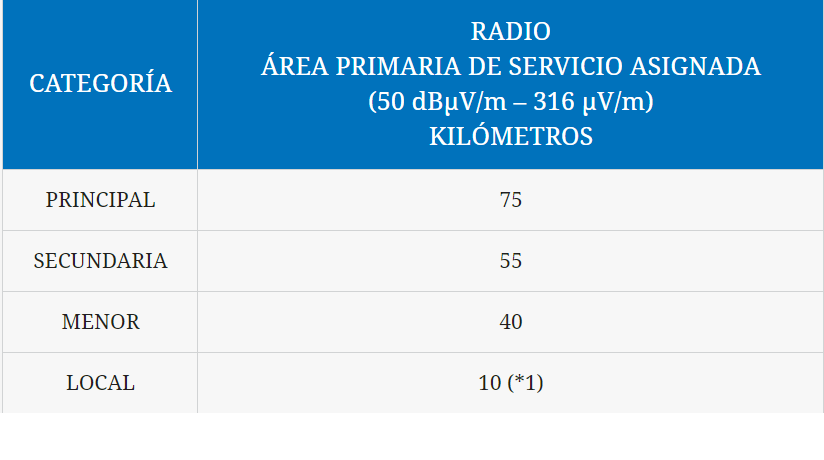
\includegraphics[width=\textwidth]{/ImagenesEjercicio5-6y7/ctt.png}
	\caption{}	
	\label{fig:ctt}
\end{figure}
